% Tento soubor nahraďte vlastním souborem s obsahem práce.
%=========================================================================
% Autoři: Michal Bidlo, Bohuslav Křena, Jaroslav Dytrych, Petr Veigend a Adam Herout 2019

% Pro kompilaci po částech (viz projekt.tex), nutno odkomentovat a upravit
%\documentclass[../projekt.tex]{subfiles}
%\begin{document}

\chapter{Úvod}
\textbf{DNS resolver} je lokálny agent, ktorý je zodpovedný za dotazovanie DNS serverov a spracovávanie odpovedí za účelom prekladu doménového mena/IP adresy alebo získavaním iných informácií spojených s doménovým menom. Umožňuje tak užívateľom rýchlešiu a jednoduchšiu navigáciu na internete.~\cite{RFC1035}

DNS resolver pracuje s distribuovaným, hierarchickým, stromovým doménovým priestorom. Tento priestor je rozdelený na \textbf{zóny}. Najvyšší bod hierarchie je \textbf{root DNS server}, ktorý obsahuje informácie o serveroch najvyššej úrovni (TLD - Top Level Domain), ktoré sú zodpovedné za správu domén pod nimi. Každá doména najvyššej úrovne má svojho správcu, ktorý je zodpovedný za správu domén pod ňou. Tento proces sa opakuje až na úroveň \textbf{autoritatívnych DNS serverov}, ktoré vykonávajú mapovanie názvu domény na adresu pre doménu danej organizácie. Bližší popis doménového priestoru možno nájsť \href{https://www.rfc-editor.org/rfc/rfc1034.txt}{tu}.

Užívateľské programy interagujú s priestorom doménových mien pomocou resolveru. Resolver odpovedá na užívateľské dopyty informáciami, ktoré získa prostredníctvom dopytov na doménové servery a miestnu vyrovnávaciu pamäť. Na základe metód vyhľadávania možno DNS resolvery rozdeliť:
\begin{itemize}
    \item Iteratívny - dotazuje niekoľko DNS serverov v hierarchickej štruktúre doménového priestoru. Tento proces sa opakuje až kým resolver nedostane záznam z autoritatívneho servera pre danú doménu.
    \begin{figure}[ht]
        \centering     % Center the image horizontally
        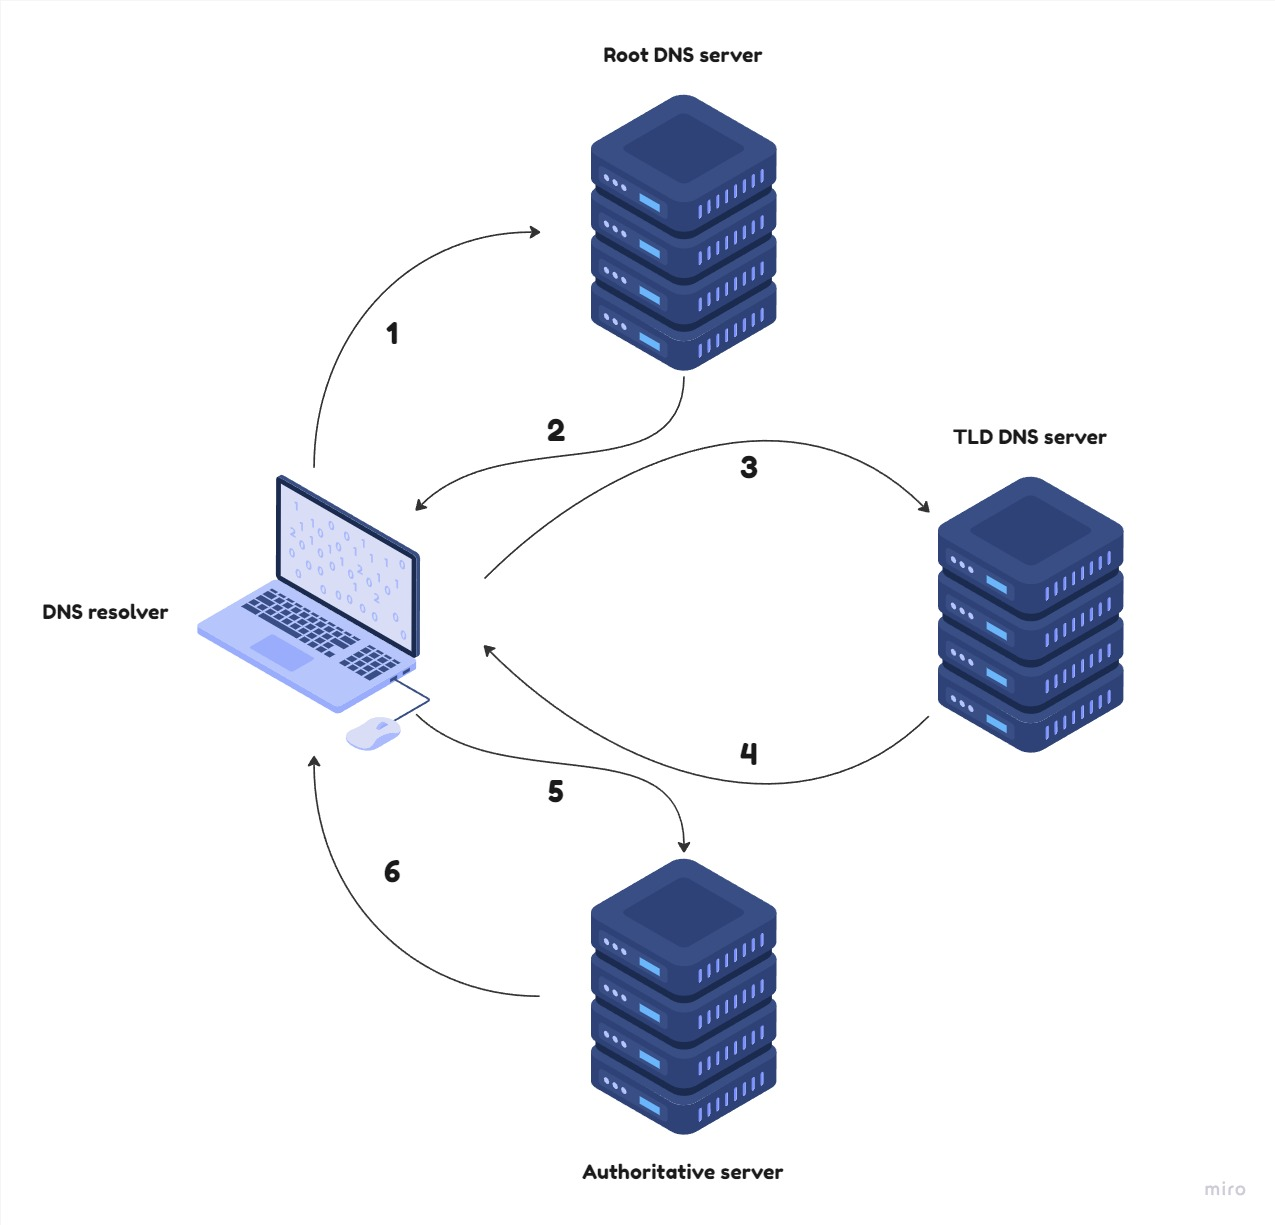
\includegraphics[width=0.6\textwidth]{obrazky-figures/Iterative.jpg}
        \caption{DNS resolver aplikujúci iteratívne dotazovanie}
        \label{fig:iterative-DNS-resolver}
    \end{figure}
    
    \item Ne-rekurzívny - dotazuje jeden DNS server, ktorý buď poskytne záznam z autoritatívneho serveru alebo čiastočnú odpoveď, bez toho, aby pokračoval v dotazovaní ďalších DNS serverov.
    
    \item Rekurzívny - dotazuje jeden DNS server, ktorý môže následne dotazovať ďalšie DNS servery. Tento proces na rozdiel od ne-rekurzívneho poskytuje kompletné riešenie pre danú doménu
    
    \begin{figure}[ht]
        \centering     % Center the image horizontally
        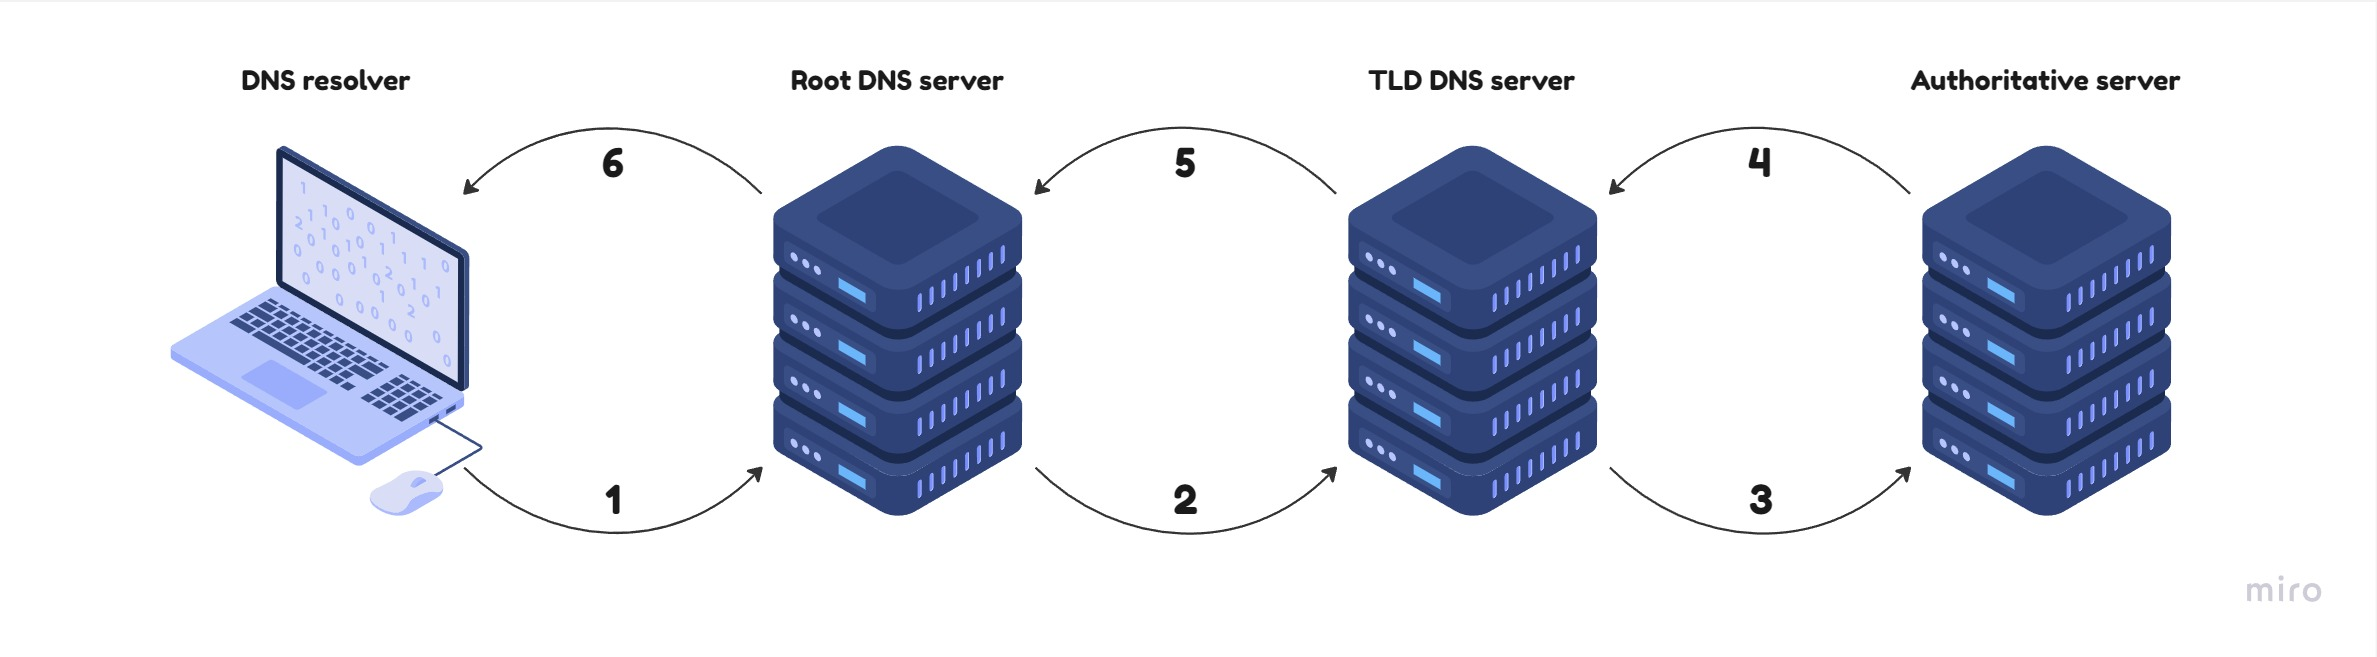
\includegraphics[width=0.6\textwidth]{obrazky-figures/Recursive.jpg}
        \caption{DNS resolver aplikujúci rekurzívne dotazovanie}
        \label{fig:your-label}
    \end{figure}
\end{itemize}



\chapter{Návrh aplikácie}

\chapter{Popis implementácie}

\section{Spracovanie argumentov}
Pre spacovanie argumentov programu som použil knižnicu \textbf{getopt.h}. Táto knižnica umožňuje definovať argumenty programu a ich spracovanie. V prípade, že programu neboli predané argumenty, alebo boli predané argumenty, ktoré nie sú definované, program vypíše nápovedu a ukončí sa. V prípade, že boli predané argumenty, ktoré sú definované, program ich spracuje a uloží do štruktúry \textbf{s\_Arguments}. Táto štruktúra obsahuje všetky argumenty, ktoré program podporuje.

Argumenty a prepínače, ktoré program podporuje sú:
\begin{itemize}
    \item \textbf{-h} - vypíše nápovedu
    \item \textbf{-r} - rekurzívne dotazovanie
    \item \textbf{-x} - inverzné dotazovanie
    \item \textbf{-6} - dotazovanie na IPv6 adresy
    \item \textbf{-s server} - adresa DNS servera, na ktorý sa bude dotazovať, povinný argument
    \item \textbf{-p port} - port DNS servera, na ktorý sa bude dotazovať, predvolená hodnota je 53
    \item \textbf{adresa} - doménové meno/IP adresa, na ktorú sa bude dotazovať, povinný argument
\end{itemize}

Poznámka ku kombinácií argumentov -x a -6 - v prípade, že sú tieto argumenty kombinované, program vypíše varovnú hlášku o ignorovaní argumentu -6 a pokračuje v spracovaní.

\section{Komunikácia so DNS serverom}
Dotazovanie na DNS server je implementované v \texttt{main} funkcii. Tu je natavený socket pre UDP komunikáciu. O zaslanie a prijatie dotazu sa starajú funkcia \texttt{sendto()}, resp. \texttt{recvfrom()}. V prípade, že sa nepodarí zaslať dotaz, alebo prijať odpoveď, program vypíše chybovú hlášku a ukončí sa.

Zostavovaniu jednotlivých častí DNS dotazu sa venujú nasledujúce sekcie.

\section{DNS hlavička a dotaz}
Zostavenie DNS hlavičky a nastavenie dotazu je zabezpečené vo funkcii \texttt{create\_DNS\_query}. Tu dochádza k naplneniu hodnôt v štruktúre hlavičky \texttt{DNS\_header} a nastavenie dotazu v štruktúre \texttt{DNS\_question}. Štruktúry som vytváral podľa definícií v sekcií 4.1. Format v~\cite{RFC1035}.

\section{Prevod doménových mien do DNS formátu(QNAME)}
O prevod doménového mena na DNS formát(Query Name) sa stará \texttt{hostname\_to\_qname} funkcia. Táto funkcia rozdelí doménové meno na jednotlivé časti, ktoré sú oddelené znakom \uv{.} a pridá k nim dĺžku danej časti. Tento postup je opakovaný až kým nie je celé doménové meno prevedené na DNS formát.

\section{Reverzné dotazovanie}
V programe je podpora pre reverzné dotazovanie IPv4 aj IPv6 adries. Dve funkcie, a to \texttt{reverse\_ipv4\_address} a \texttt{reverse\_ipv6\_address}, slúžia na prevod IPv4 a IPv6 adries na doménové mená. Následne už stačí len zavolať funkciu \texttt{hostname\_to\_qname} a doménové meno je pripravené na dotazovanie.




\begin{gather*}
    \texttt{www.seznam.cz -> 3www5seznam2cz0}
\end{gather*}



\chapter{Použitie}
